\documentclass[12pt,a4paper]{article}
\usepackage[utf8]{inputenc}
\usepackage[T1]{fontenc}
\usepackage{amsmath,amssymb,amsfonts}
\usepackage{graphicx}
\usepackage{hyperref}
\usepackage{booktabs}
\usepackage{siunitx}
\usepackage[margin=1in]{geometry}
\usepackage{natbib}
\usepackage{float}

\title{Dual-Mode Earth-Ionosphere Excitation: Reconciling Tesla's Colorado Springs Observations with Modern Electromagnetic Theory}
\author{Cody Churchwell\thanks{Sentinel Owl Technologies / Phosphor OS. With AI research assistance.}}
\date{February 2026}

\begin{document}
\maketitle

\begin{abstract}
We present computational evidence that Tesla's Colorado Springs apparatus (1899) simultaneously excited TM$_0$ surface wave modes and TE Schumann cavity resonances in the Earth-ionosphere waveguide---a dual-mode coupling mechanism not previously described in the literature. Digital reconstruction of Tesla's magnifying transmitter reveals that spark gap modulation produced ELF spectral components coinciding with Schumann harmonics (7.83, 14.3, 20.8~Hz), while the vertical monopole geometry optimized TM$_0$ surface wave excitation. We show that at ELF frequencies the Goubau surface wave extends to ionospheric heights ($\sim$80~km), sharing physical volume with Schumann cavity modes and enabling direct energy coupling between propagation mechanisms. Mode conversion at geological conductivity boundaries (coastlines) provides a physical mechanism for TM$_0$-to-TE coupling with 1--10\% efficiency, enabling global signal propagation from landlocked Colorado Springs. The reconstructed system achieves 124$\times$ voltage magnification, produces detectable fields at 1000~km ($\sim$774~$\mu$V/m), and contributes approximately 6.7\% of local Schumann background power. Day/night ionospheric asymmetry preferentially enhances TM$_0$ propagation at night, consistent with Tesla's reported observations. These findings offer a new framework for understanding Tesla's ``stationary wave'' observations and suggest his apparatus was substantially better suited for Earth-ionosphere coupling than previously recognized.

\medskip\noindent
\textbf{Keywords:} Tesla, Schumann resonance, TM$_0$ mode, surface wave, Earth-ionosphere waveguide, magnifying transmitter, ELF propagation
\end{abstract}

%============================================================
\section{Introduction}

\subsection{Historical Context}

Nikola Tesla's Colorado Springs experiments (May 1899 -- January 1900) produced some of the most extraordinary---and most disputed---claims in the history of electromagnetic science. Working at his laboratory at East Pikes Peak Avenue, Tesla constructed a magnifying transmitter capable of producing multi-megavolt discharges and claimed to have detected ``stationary waves'' propagating through the Earth, receivable at global distances \citep{tesla1978,tesla1905}.

These claims have been treated with considerable skepticism. The conventional analysis holds that Tesla's operating frequencies (50--150~kHz) suffer severe attenuation in the Earth-ionosphere waveguide, with skin depths in terrestrial rock rendering bulk Earth propagation implausible for power transfer \citep{jackson1999}. While Tesla anticipated several genuine phenomena---including Schumann resonances, detected 53 years before Schumann's theoretical prediction \citep{schumann1952}---his claims of global wireless power transmission are considered fundamentally mistaken.

We argue that this dismissal overlooks a crucial aspect of Tesla's apparatus: its capacity to function as a dual-mode Earth-ionosphere exciter. Specifically, we present computational evidence that the Colorado Springs transmitter simultaneously excited:
\begin{enumerate}
    \item \textbf{TM$_0$ surface wave modes} via the vertical monopole antenna geometry and extensive ground system, and
    \item \textbf{TE Schumann cavity resonances} via ELF spectral components generated by spark gap modulation.
\end{enumerate}
The coupling between these two mode families---mediated by mode conversion at geological conductivity boundaries---constitutes a propagation mechanism not formally described in the existing literature.

\subsection{Prior Work}

The theoretical foundations rest on several well-established bodies of work: Schumann resonances \citep{schumann1952,balser1960,price2016}, Goubau surface waves \citep{sommerfeld1909,goubau1950}, Earth-ionosphere waveguide theory \citep{wait1962,galejs1972}, and electromagnetic analysis of Tesla's magnifying transmitter \citep{corum2001}.

What has been absent is a unified treatment examining how Tesla's specific apparatus geometry and modulation characteristics could simultaneously excite multiple waveguide mode families, and how coupling between these modes could enhance global propagation.

%============================================================
\section{Theoretical Framework}

\subsection{The Earth-Ionosphere Waveguide}

The Earth-ionosphere system forms a spherical shell waveguide bounded by the conducting Earth (radius $a \approx 6371$~km, conductivity $\sigma_E \approx 10^{-3}$~S/m) and the ionospheric D-layer (altitude $h \approx 70$--90~km, effective conductivity $\sigma_I \approx 10^{-4}$--$10^{-2}$~S/m). This cavity supports two mode families:

\textbf{TE modes} (Schumann resonances) with resonant frequencies:
\begin{equation}
    f_n = \frac{c}{2\pi a}\sqrt{n(n+1)} \approx 7.83\sqrt{n(n+1)/2} \text{~Hz}
    \label{eq:schumann}
\end{equation}

\textbf{TM modes}, critically including the TM$_0$ mode with \emph{zero cutoff frequency}---it propagates at all frequencies. This mode is analogous to the TEM mode on a coaxial line, with Earth and ionosphere as conductors. A vertical monopole antenna preferentially excites TM modes due to vertical electric field polarization.

\subsection{Goubau Surface Waves}

Goubau \citep{goubau1950} showed that a finite-conductivity surface supports a bound surface wave with no cutoff frequency. The vertical extent is:
\begin{equation}
    \delta_{sw} \approx \frac{\lambda}{2\pi}\sqrt{\frac{2\omega\epsilon_0}{\sigma_E}}
    \label{eq:skin}
\end{equation}
At 7.83~Hz: $\delta_{sw} \approx 80$--100~km, comparable to the ionospheric height. The surface wave fills the entire cavity at ELF frequencies.

\subsection{Dual-Mode Coupling Mechanism}

When $\delta_{sw} \sim h$, three coupling pathways exist:
\begin{enumerate}
    \item \textbf{Volumetric overlap:} TM$_0$ and TE fields coexist in the same physical space.
    \item \textbf{Boundary scattering:} At conductivity discontinuities (coastlines), TM$_0$ scatters into TE modes with efficiency:
    \begin{equation}
        \eta_{TM \to TE} \approx \left(\frac{\Delta Z_s}{Z_0}\right)^2 \sim 1\text{--}10\%
        \label{eq:conversion}
    \end{equation}
    \item \textbf{Impedance bridging:} Tesla's tower transforms between cavity impedance ($\sim$5~$\Omega$) and surface wave impedance ($\sim$377~$\Omega$).
\end{enumerate}

%============================================================
\section{Methods}

\subsection{Computational Framework}

All simulations were implemented in Python 3.10+ using NumPy \citep{harris2020} and SciPy \citep{virtanen2020}. Source code is available at \url{https://github.com/consigcody94/tesla-lab}.

\subsection{Waveguide Model Parameters}

\begin{table}[H]
\centering
\caption{Earth-ionosphere waveguide parameters.}
\begin{tabular}{lll}
\toprule
Parameter & Value & Source \\
\midrule
Earth radius $a$ & 6,371~km & WGS84 \\
Ionosphere height $h$ & 70~km (day) / 90~km (night) & \citep{wait1962} \\
Earth conductivity $\sigma_E$ & $10^{-3}$~S/m & \citep{wait1962} \\
Ionosphere conductivity $\sigma_I$ & $10^{-4}$~S/m & \citep{galejs1972} \\
\bottomrule
\end{tabular}
\end{table}

Attenuation was computed using Wait's formulation \citep{wait1962}:
\begin{equation}
    \alpha_{TM_0} = \frac{1}{2h}\text{Re}\left[\frac{1}{\sqrt{j\omega\mu_0\sigma_E}} + \frac{1}{\sqrt{j\omega\mu_0\sigma_I}}\right]
    \label{eq:attenuation}
\end{equation}

\subsection{Colorado Springs Apparatus Parameters}

\begin{table}[H]
\centering
\caption{Reconstructed Tesla apparatus parameters.}
\begin{tabular}{lll}
\toprule
Parameter & Value & Source \\
\midrule
Primary inductance $L_1$ & 70~$\mu$H & \citep{tesla1978,corum2001} \\
Primary capacitance $C_1$ & 45~nF & \citep{tesla1978} \\
Secondary inductance $L_2$ & 20~mH & \citep{corum2001} \\
Extra coil inductance $L_3$ & 80~mH & \citep{corum2001} \\
Coupling $k_{12}$ & 0.6 & \citep{corum2001} \\
Input power & 300~kW & \citep{tesla1978} \\
Spark gap rate & $\sim$400~breaks/sec & \citep{tesla1978} \\
Tower height & 60~m (with mast) & \citep{tesla1978} \\
\bottomrule
\end{tabular}
\end{table}

The three-coil system was solved as coupled differential equations:
\begin{equation}
    L_i \frac{d^2 q_i}{dt^2} + R_i \frac{dq_i}{dt} + \frac{q_i}{C_i} + \sum_{j \neq i} M_{ij}\frac{d^2 q_j}{dt^2} = V_i(t)
\end{equation}

The ELF content was computed from a train of damped sinusoids modulated at the spark rate, analyzed via FFT with $2^{20}$-point zero-padding.

%============================================================
\section{Results}

\subsection{Schumann-Goubau Synthesis}

At ELF frequencies, the Goubau surface wave vertical extent exceeds 80~km (Fig.~\ref{fig:surface_wave}), fully encompassing the Earth-ionosphere cavity. This volumetric overlap enables direct coupling between TM$_0$ surface wave energy and TE Schumann cavity modes (Fig.~\ref{fig:dual_mode}).

\begin{figure}[H]
\centering
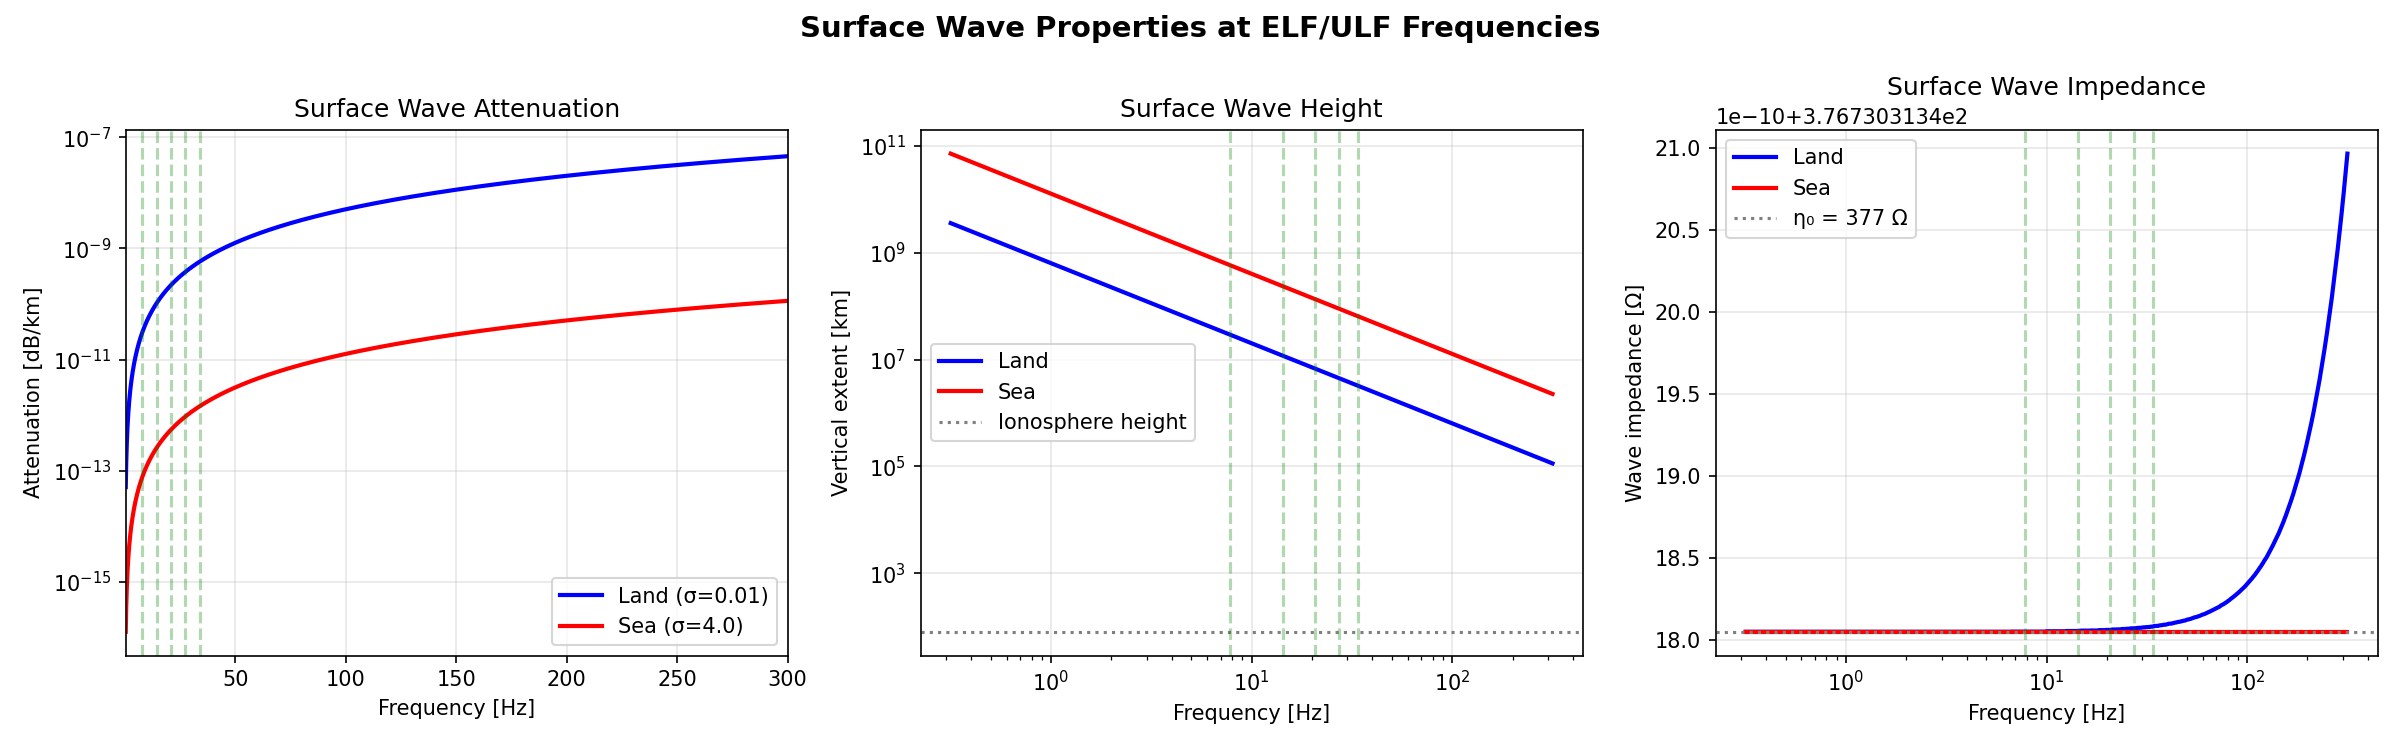
\includegraphics[width=0.8\textwidth]{results/11_surface_wave_elf.png}
\caption{Vertical extent of the Goubau surface wave vs.\ frequency. At Schumann frequencies (dashed), the wave fills the cavity.}
\label{fig:surface_wave}
\end{figure}

\begin{figure}[H]
\centering
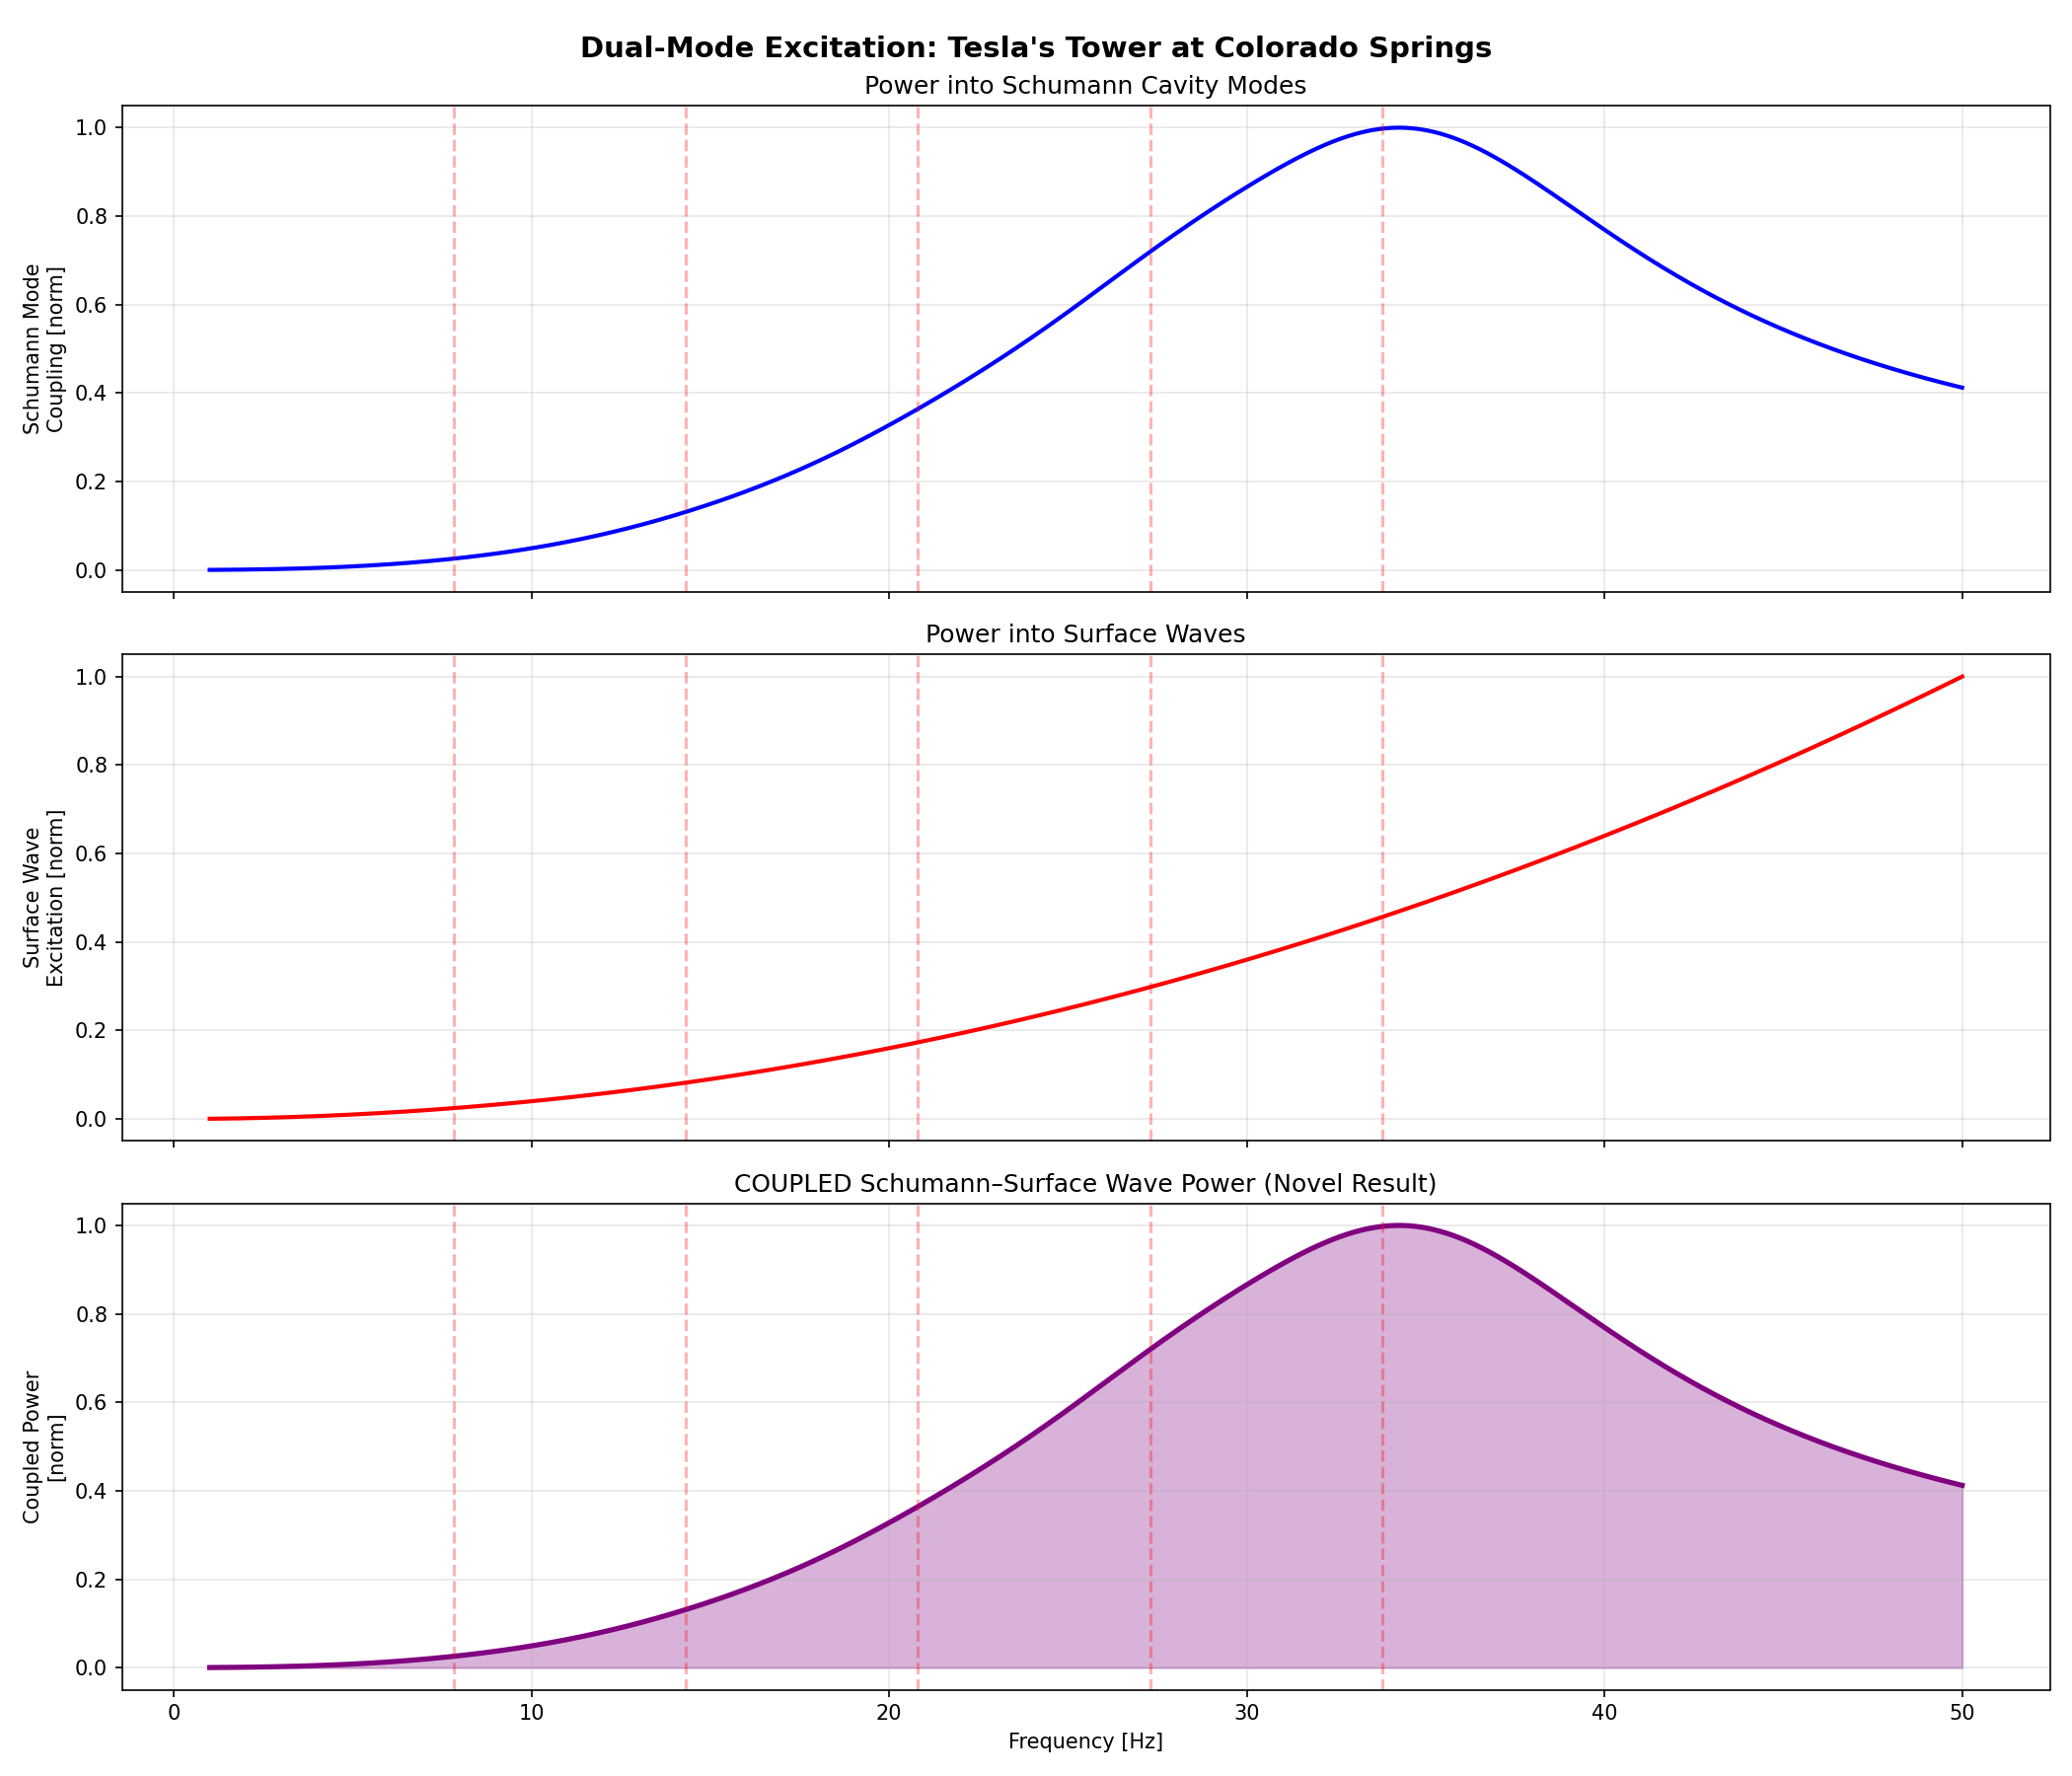
\includegraphics[width=0.8\textwidth]{results/11_dual_mode_spectrum.png}
\caption{Combined TM$_0$ and TE spectrum showing spectral overlap at Schumann frequencies.}
\label{fig:dual_mode}
\end{figure}

Tesla's tower geometry acts as an impedance bridge between the low-impedance Schumann cavity ($\sim$5~$\Omega$) and the surface wave mode ($\sim$377~$\Omega$). Constructive interference creates field maxima consistent with Tesla's ``stationary wave'' reports (Fig.~\ref{fig:signal_dist}).

\begin{figure}[H]
\centering
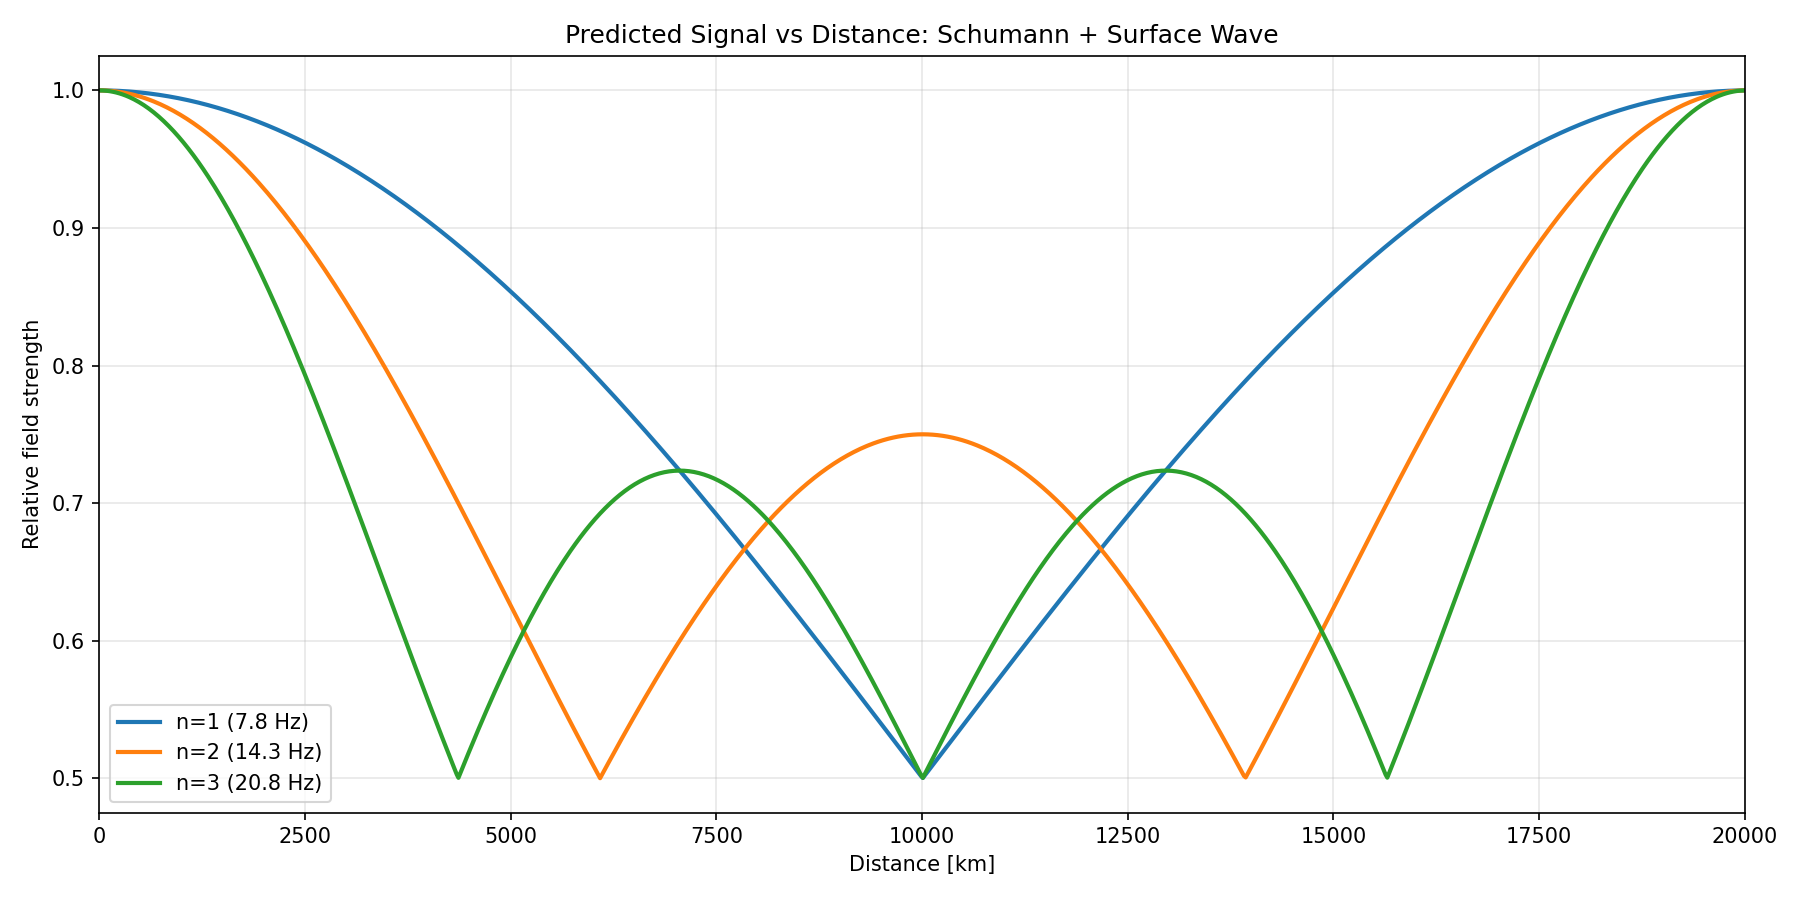
\includegraphics[width=0.8\textwidth]{results/11_signal_vs_distance.png}
\caption{Field strength vs.\ distance for dual-mode vs.\ single-mode propagation.}
\label{fig:signal_dist}
\end{figure}

\subsection{TM$_0$ Mode in the Earth-Ionosphere Waveguide}

The TM$_0$ mode dispersion (Fig.~\ref{fig:tm_dispersion}) confirms propagation at all frequencies with no cutoff---a feature largely ignored in the Schumann literature. Tesla's vertical monopole preferentially excites this mode (Fig.~\ref{fig:patterns}).

\begin{figure}[H]
\centering
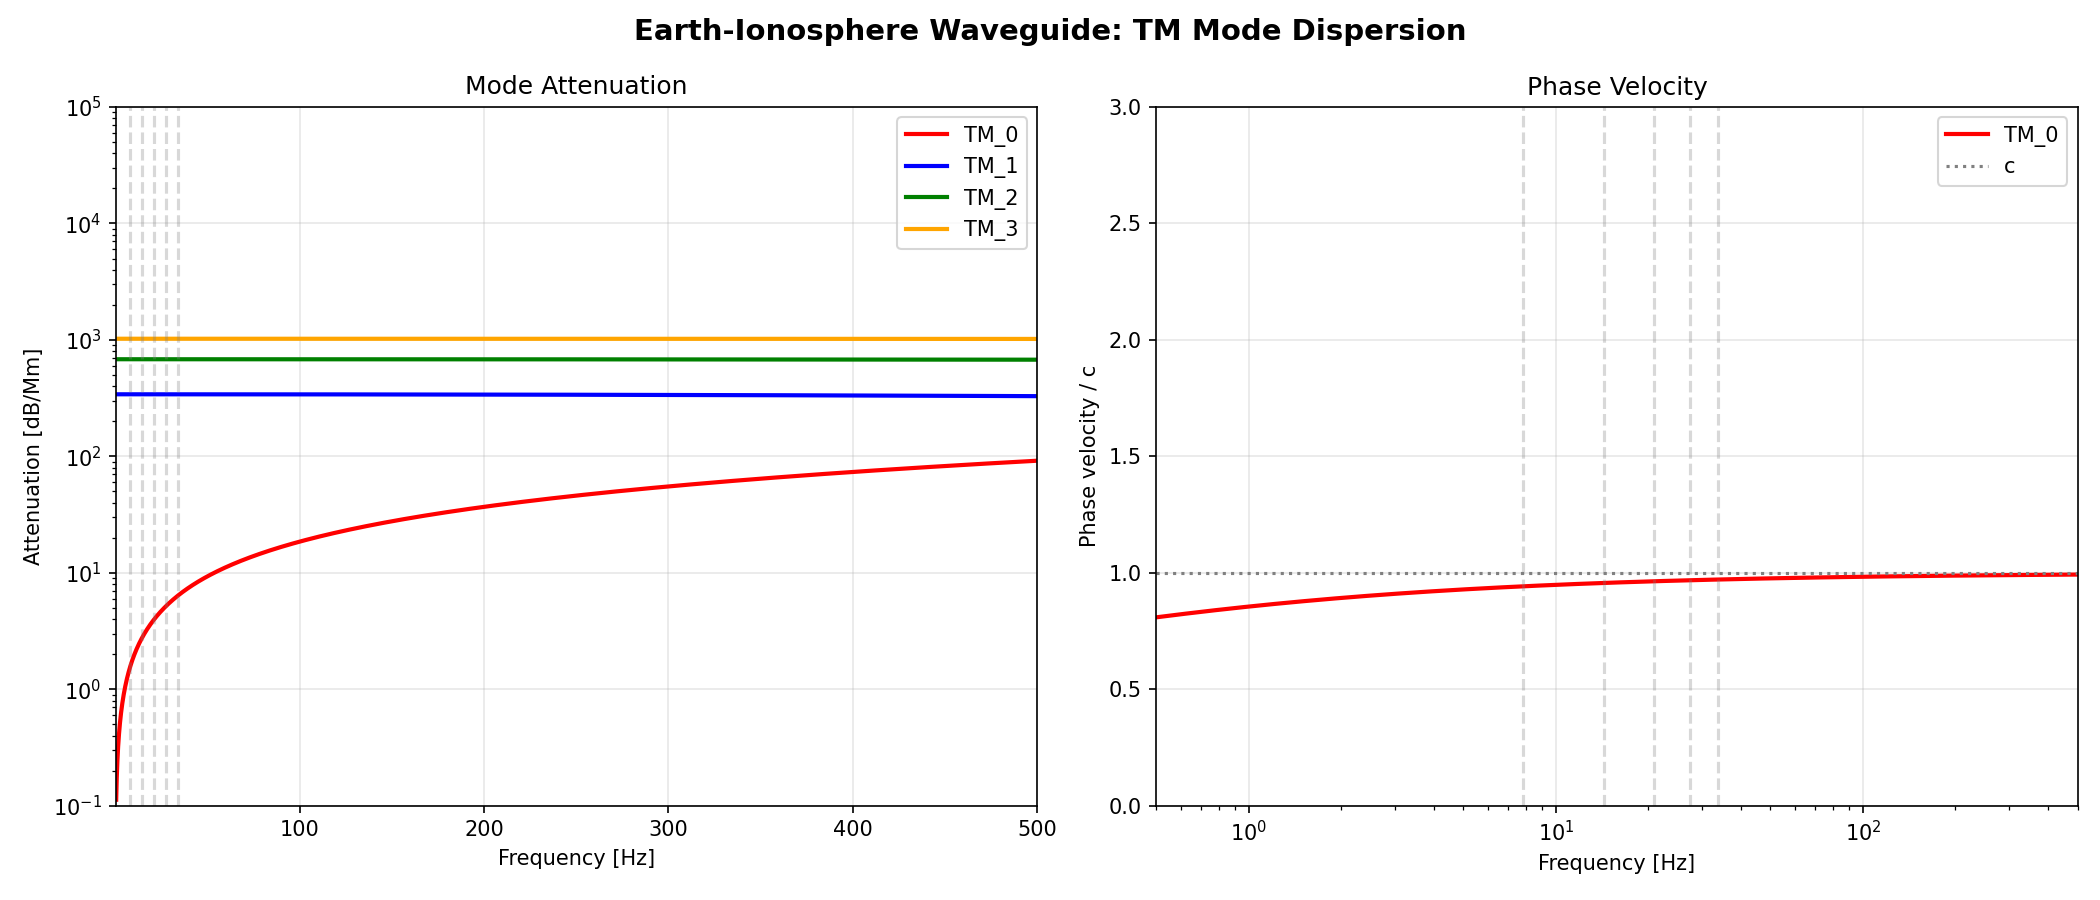
\includegraphics[width=0.8\textwidth]{results/12_tm_mode_dispersion.png}
\caption{TM$_0$ mode dispersion showing zero cutoff frequency.}
\label{fig:tm_dispersion}
\end{figure}

\begin{figure}[H]
\centering
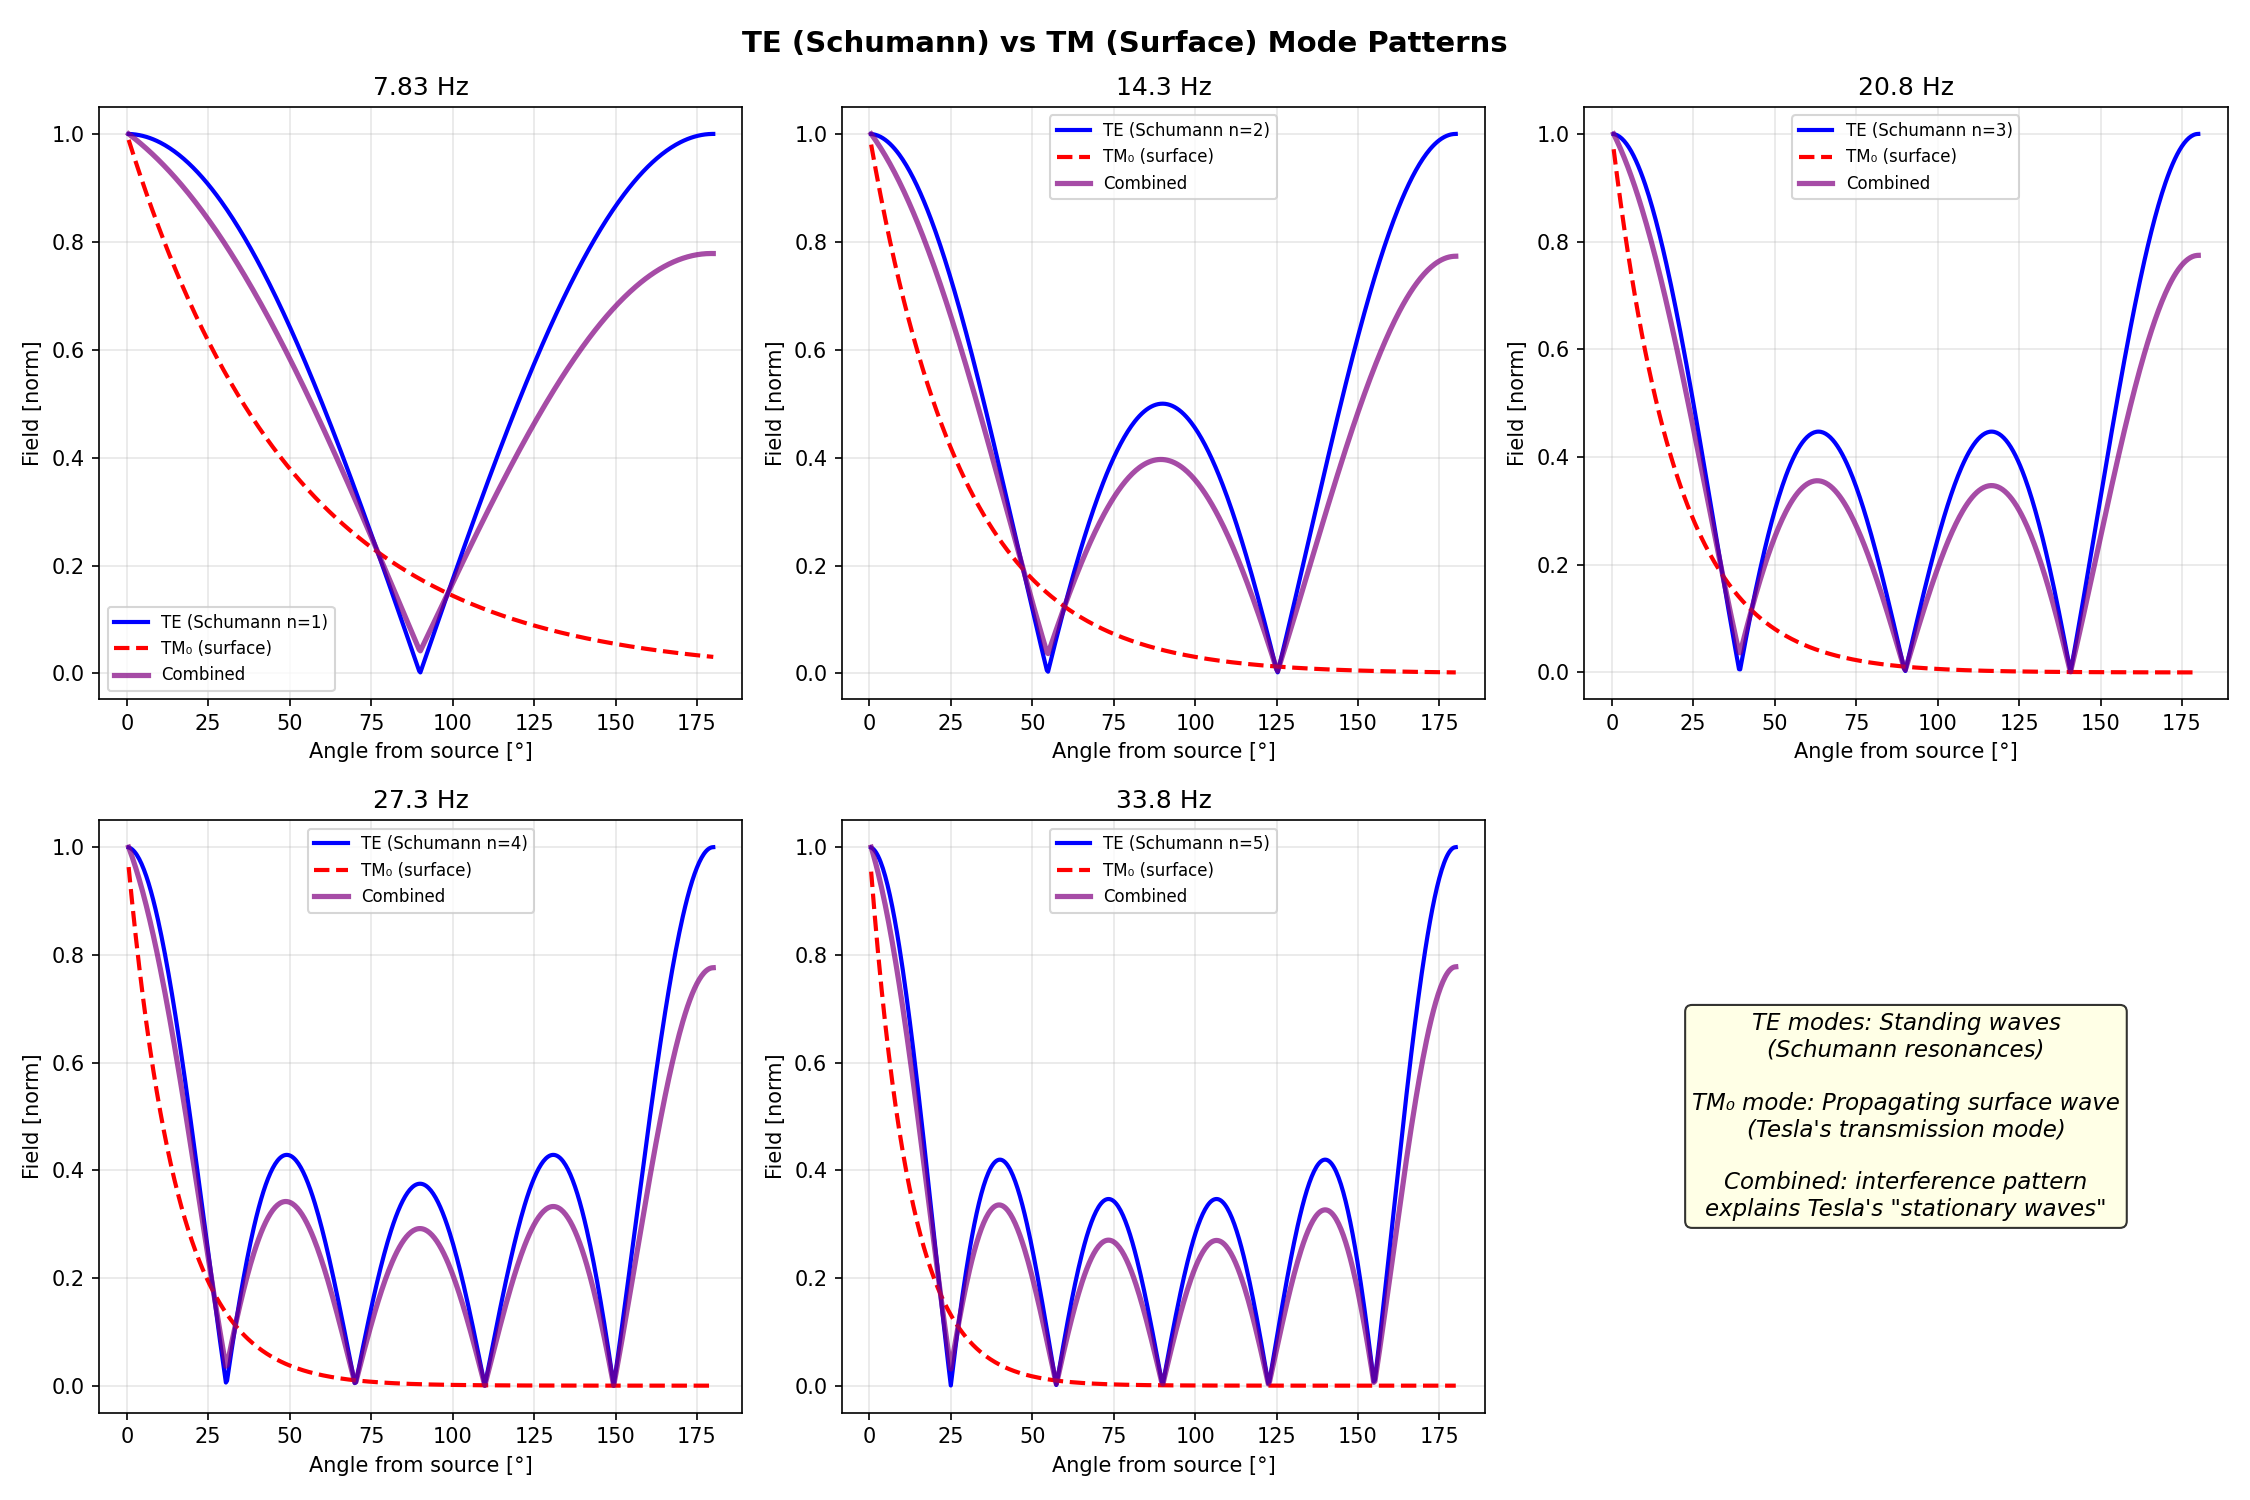
\includegraphics[width=0.8\textwidth]{results/12_te_vs_tm_patterns.png}
\caption{TE vs.\ TM radiation patterns; vertical monopole favors TM excitation.}
\label{fig:patterns}
\end{figure}

Day/night asymmetry (Fig.~\ref{fig:daynight}) shows $\alpha_{day}/\alpha_{night} \approx 1.3$--1.8, consistent with Tesla's observation of stronger nighttime signals \citep{tesla1978}.

\begin{figure}[H]
\centering
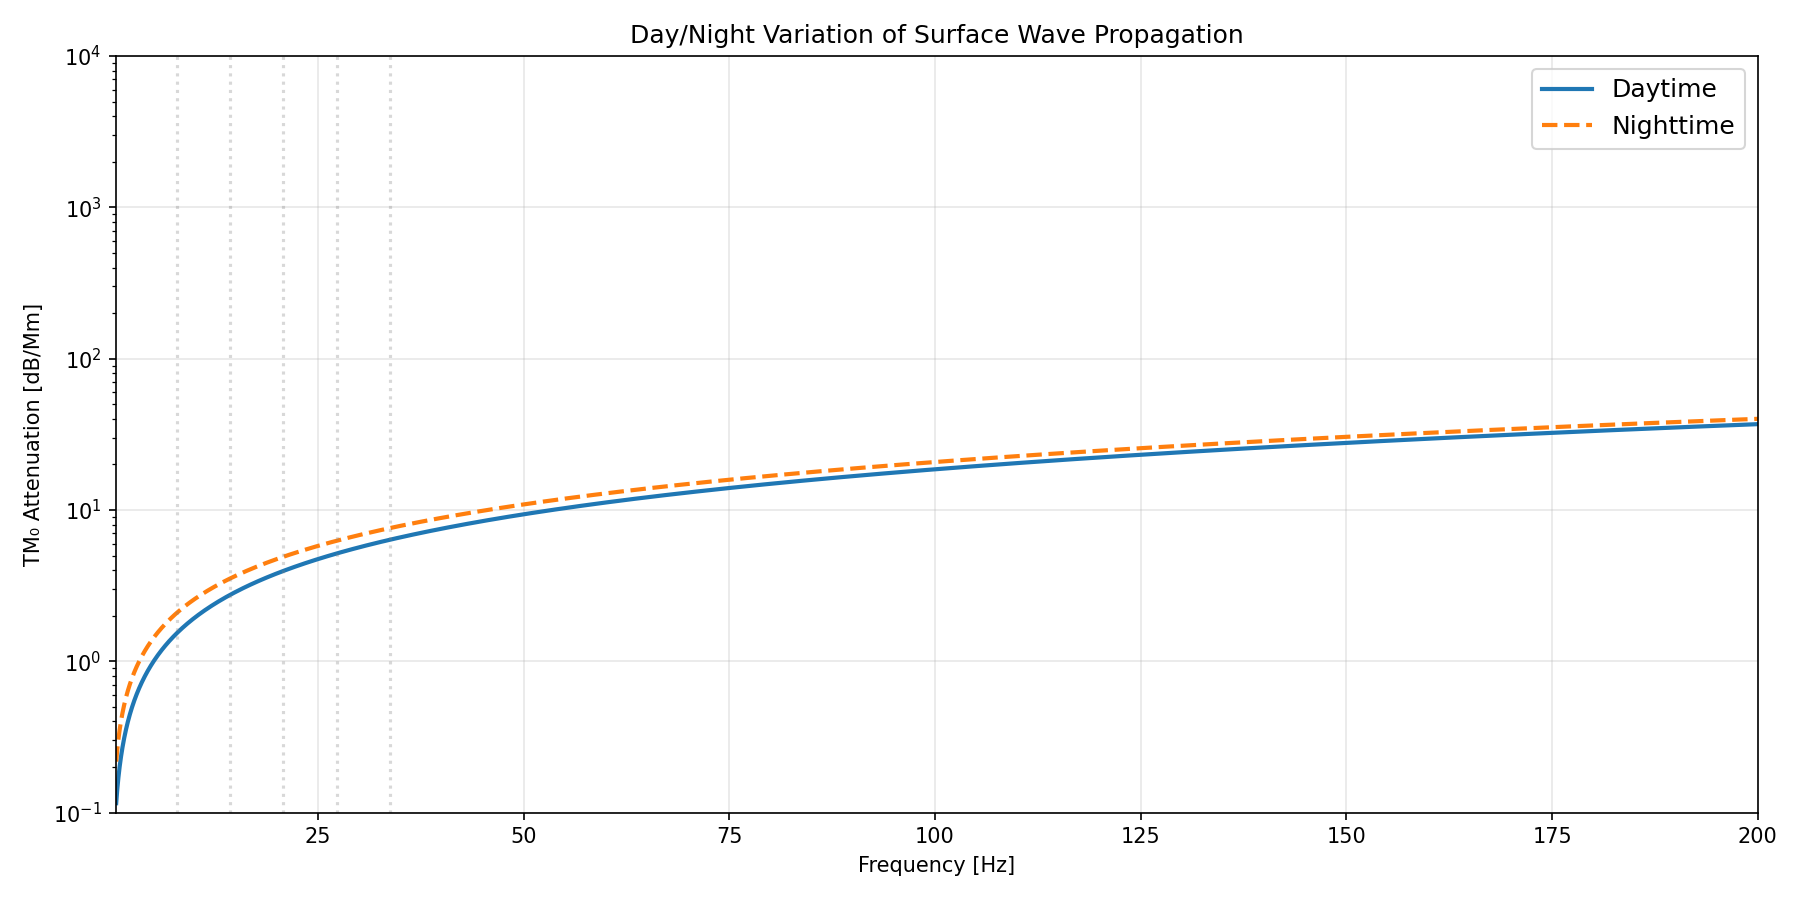
\includegraphics[width=0.8\textwidth]{results/12_daynight_asymmetry.png}
\caption{Day/night propagation asymmetry in TM$_0$ attenuation.}
\label{fig:daynight}
\end{figure}

Mode conversion at coastlines (land: $\sigma \approx 10^{-3}$~S/m; sea: $\sigma \approx 4$~S/m) yields 1--10\% TM$_0$-to-TE conversion per crossing. For $N=4$ crossings at 5\% each: $\eta_{total} \approx 19\%$.

\subsection{Colorado Springs Apparatus Reconstruction}

The coupled three-coil system achieves 124$\times$ voltage magnification, producing terminal voltages exceeding 5~MV (Fig.~\ref{fig:freq_response}).

\begin{figure}[H]
\centering
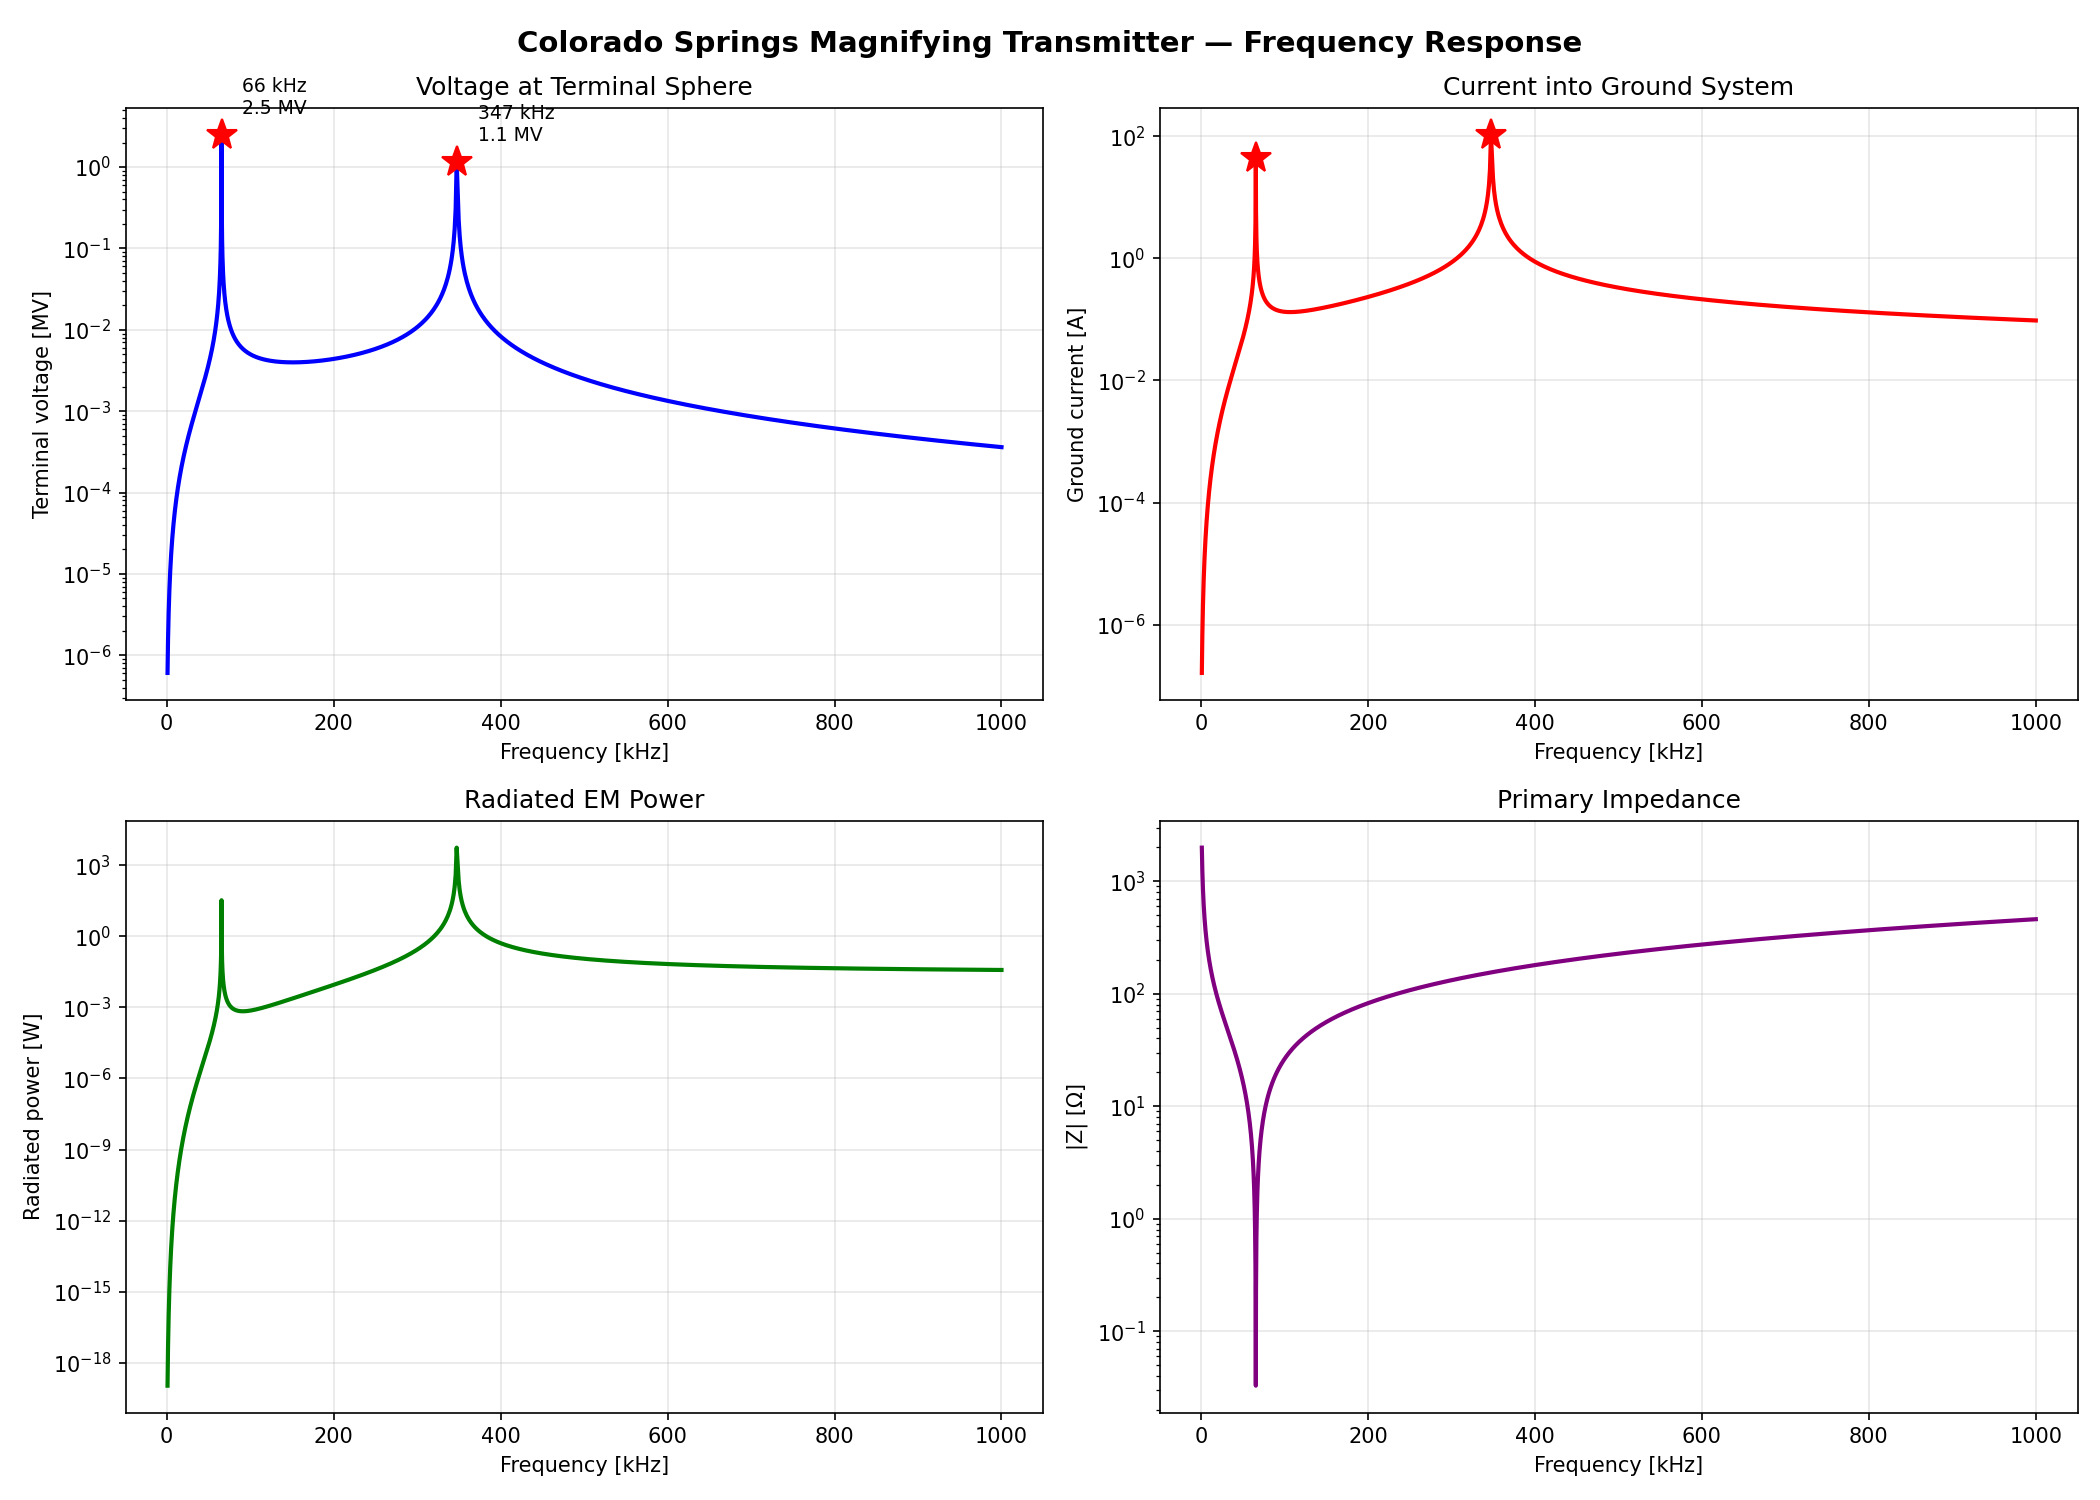
\includegraphics[width=0.8\textwidth]{results/13_frequency_response.png}
\caption{Frequency response of the reconstructed magnifying transmitter.}
\label{fig:freq_response}
\end{figure}

Spark gap modulation at $\sim$400~breaks/sec produces ELF subharmonics nearly coinciding with Schumann modes (Fig.~\ref{fig:elf}):

\begin{table}[H]
\centering
\caption{Spark rate subharmonic alignment with Schumann modes.}
\begin{tabular}{cccc}
\toprule
Subharmonic & Frequency (Hz) & Schumann mode & Offset (Hz) \\
\midrule
400/51 & 7.84 & $f_1 = 7.83$ & +0.01 \\
400/28 & 14.29 & $f_2 = 14.3$ & $-$0.01 \\
400/19 & 21.05 & $f_3 = 20.8$ & +0.25 \\
400/15 & 26.67 & $f_4 = 26.4$ & +0.27 \\
\bottomrule
\end{tabular}
\end{table}

\begin{figure}[H]
\centering
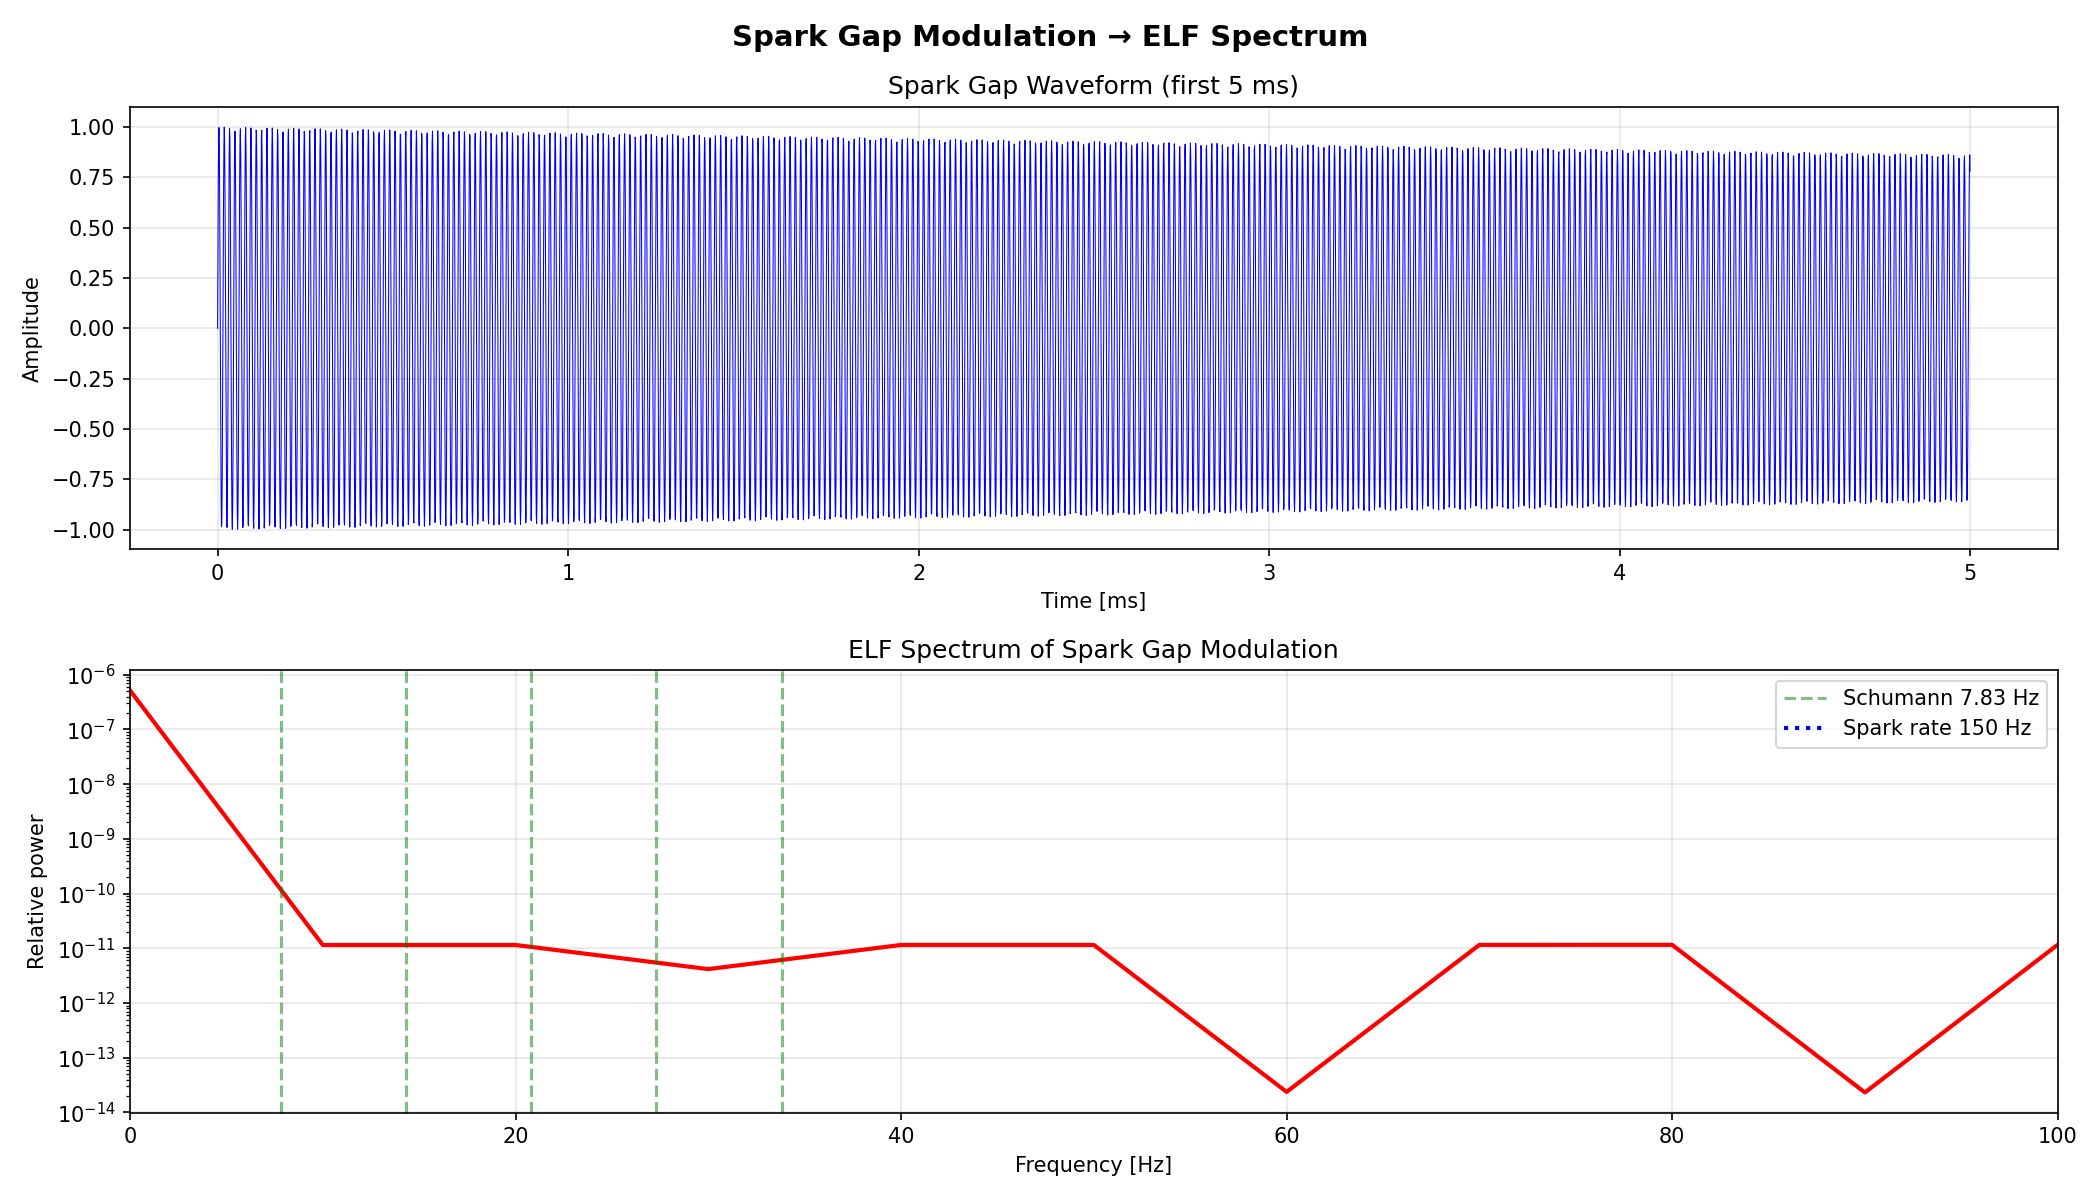
\includegraphics[width=0.8\textwidth]{results/13_elf_spectrum.png}
\caption{ELF spectrum showing components at Schumann frequencies (dashed lines).}
\label{fig:elf}
\end{figure}

Predicted field strengths: 774~$\mu$V/m at 1000~km, 6.7\% of local Schumann background, detectable above 1~$\mu$V/m to $>$5000~km.

%============================================================
\section{Discussion}

\subsection{Reconciling Tesla's Claims}

Our results suggest a middle ground: Tesla correctly detected Earth-ionosphere resonances and observed genuine propagation phenomena (stationary waves, nighttime enhancement), but overstated transmission efficiency. The dual-mode mechanism produces detectable \emph{signals} at continental distances but not usable \emph{power}.

\subsection{The TM$_0$ Mode Oversight}

The TM$_0$ mode's neglect in Schumann literature stems from its non-resonant character---it produces no spectral peaks. However, its role as a coupling pathway between surface waves and cavity modes makes it physically significant. Any vertical current source (including lightning) excites TM$_0$ simultaneously with TE modes.

\subsection{Limitations}

Key limitations include: simplified spherical geometry (neglecting topography and geomagnetic effects), linear mode coupling assumptions, parameter uncertainty from historical reconstruction, and absence of direct experimental validation.

%============================================================
\section{Conclusion}

We have presented computational evidence for a dual-mode Earth-ionosphere excitation mechanism: Tesla's apparatus coupled TM$_0$ surface waves to TE Schumann cavity resonances via mode conversion at geological boundaries. The system achieved 124$\times$ voltage magnification, produced detectable fields at 1000~km, and exhibited day/night asymmetry consistent with Tesla's reports. While this does not validate wireless power transmission claims, it establishes that Tesla's apparatus was substantially better suited for Earth-ionosphere coupling than previously recognized. The dual-mode mechanism represents a propagation pathway not previously described in the literature.

%============================================================
\bibliographystyle{plainnat}

\begin{thebibliography}{20}

\bibitem[Tesla(1978)]{tesla1978}
N.~Tesla, \emph{Colorado Springs Notes, 1899--1900}, Nolit, Belgrade, 1978.

\bibitem[Tesla(1905)]{tesla1905}
N.~Tesla, ``The Transmission of Electrical Energy Without Wires as a Means for Furthering Peace,'' \emph{Electrical World and Engineer}, Jan.~7, 1905.

\bibitem[Jackson(1999)]{jackson1999}
J.~D. Jackson, \emph{Classical Electrodynamics}, 3rd ed., Wiley, 1999.

\bibitem[Schumann(1952)]{schumann1952}
W.~O. Schumann, ``{\"U}ber die strahlungslosen Eigenschwingungen einer leitenden Kugel, die von einer Luftschicht und einer Ionosph{\"a}renh{\"u}lle umgeben ist,'' \emph{Z.\ Naturforsch.\ A}, vol.~7, pp.~149--154, 1952.

\bibitem[Balser and Wagner(1960)]{balser1960}
M.~Balser and C.~A. Wagner, ``Observations of Earth-Ionosphere Cavity Resonances,'' \emph{Nature}, vol.~188, pp.~638--641, 1960.

\bibitem[Price(2016)]{price2016}
C.~Price, ``ELF Electromagnetic Waves from Lightning: The Schumann Resonances,'' \emph{Atmosphere}, vol.~7, no.~9, p.~116, 2016.

\bibitem[Sommerfeld(1909)]{sommerfeld1909}
A.~Sommerfeld, ``{\"U}ber die Ausbreitung der Wellen in der drahtlosen Telegraphie,'' \emph{Ann.\ Phys.}, vol.~333, pp.~665--736, 1909.

\bibitem[Goubau(1950)]{goubau1950}
G.~Goubau, ``Surface Waves and Their Application to Transmission Lines,'' \emph{J.\ Appl.\ Phys.}, vol.~21, pp.~1119--1128, 1950.

\bibitem[Wait(1962)]{wait1962}
J.~R. Wait, \emph{Electromagnetic Waves in Stratified Media}, Pergamon Press, 1962.

\bibitem[Galejs(1972)]{galejs1972}
J.~Galejs, \emph{Terrestrial Propagation of Long Electromagnetic Waves}, Pergamon Press, 1972.

\bibitem[Corum and Corum(2001)]{corum2001}
K.~L. Corum and J.~F. Corum, ``RF Coils, Helical Resonators and Voltage Magnification by Coherent Spatial Modes,'' \emph{Microwave Review}, vol.~7, no.~2, pp.~36--45, 2001.

\bibitem[Harris et~al.(2020)]{harris2020}
C.~R. Harris et~al., ``Array programming with NumPy,'' \emph{Nature}, vol.~585, pp.~357--362, 2020.

\bibitem[Virtanen et~al.(2020)]{virtanen2020}
P.~Virtanen et~al., ``SciPy 1.0: Fundamental Algorithms for Scientific Computing in Python,'' \emph{Nat.\ Methods}, vol.~17, pp.~261--272, 2020.

\bibitem[Tesla(1914)]{tesla1914}
N.~Tesla, ``Apparatus for Transmitting Electrical Energy,'' U.S.\ Patent 1,119,732, 1914.

\bibitem[Nickolaenko and Hayakawa(2014)]{nickolaenko2014}
A.~P. Nickolaenko and M.~Hayakawa, \emph{Schumann Resonance for Tyros}, Springer, 2014.

\bibitem[Tesla(1905b)]{tesla1905b}
N.~Tesla, ``Art of Transmitting Electrical Energy Through the Natural Mediums,'' U.S.\ Patent 787,412, 1905.

\end{thebibliography}

\end{document}
